% !TEX root = ../Dokumentation.tex
\subsection{Fahrbahnerkennung}
\textbf{Umsetzung}\\[0.2cm]
Die Fahrbahnerkennung ist primär mittels Kamera realisiert. der gesamte Prozess ist in Abbildung \ref{fig:activityRoute} dargestellt. Nebst der Bildverarbeitung meldet die Fahrbahnerkennung alle notwendigen Informationen an den Controller. Eine weitere Aufgabe der Fahrbahnerkennung ist die Identifikation der Kreuzungen und des Zielfeldes.
\begin{figure}[H]%Position festigen
\centering
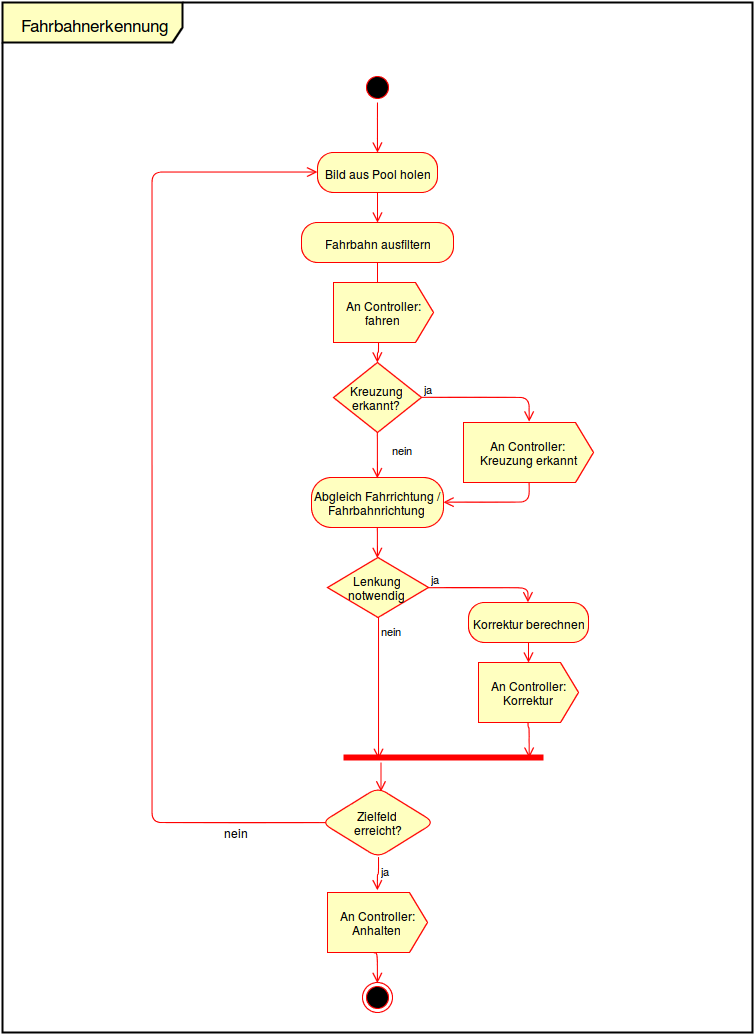
\includegraphics[width=0.7\textwidth]{03_Loesungskonzept/pictures/Fahrbahnerkennung.png}
\caption{Aktivitätendiagramm Fahrbahnerkennung}
\label{fig:activityRoute}
\end{figure}
Es wird jeweils das aktuelle Bild von der Klasse \code{PictureCreator} entnommen, mit OpenCV in Graustufen umgewandelt und anschliessend an die Kantenerkennung weitergegeben. Für die Kanten wird eine eigene Matrix erstellt, vorgelegt mit dem Graustufenwert 0. Die Kantenerkennung basiert auf der Differentialrechnung und betrachtet vom aktuellen Pixel aus in $x$ (Spalte) und $y$ (Zeile) den Graustufenwert des nächsten Pixels und des vorherigen Pixels.
$z = f(x,y) = \text{ Graustufen des Pixels }0 \leq z \leq 255$\\
\[
\frac{\partial{z}}{\partial{x}}=\frac{f(x+\Delta{x})-f(x-\Delta{x})}{2\Delta{x}} = \frac{f(x+1)-f(x-1)}{2}
\]
\[
\frac{\partial{z}}{\partial{y}}=\frac{f(y+\Delta{x})-f(y-\Delta{y})}{2\Delta{y}} = \frac{f(y+1)-f(y-1)}{2}
\]
\[
\nabla f(x,y) = \begin{bmatrix}
\frac{\partial{z}}{\partial{x}}\\
\frac{\partial{z}}{\partial{y}}
\end{bmatrix}
\]
\[
\lVert\nabla f(x,y)\rVert = \sqrt{\Biggl(\frac{\partial{z}}{\partial{x}}\Biggr)^2 + \Biggl(\frac{\partial{z}}{\partial{y}}\Biggr)^2}
\]
Übersteigt die Änderung der Graustufe den vorgegebenen Schwellwert wird eine Kante erkannt, an die entsprechende Pixelposition der Zielmatrix wird der Wert 255 geschrieben, ansonsten nicht. Der Schwellwert kann in der Konfigurationsdatei festgelegt werden und wurde mit einer Reihe von Testbildern bei unterschiedlichen Lichtverhältnissen ermittelt. Mit der festgelegten Kameraposition beschränkt sich die Fahrbahnerkennung auf die untere Bildhälfte. Damit werden störende Effekte in der Umgebung vermieden (Abbildung: \ref{fig:edges}). 
\begin{figure}[H]%Position festigen
\centering
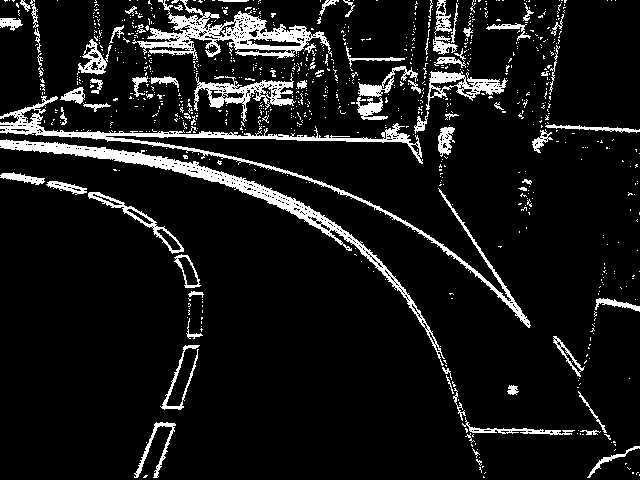
\includegraphics[width=0.6\textwidth]{03_Loesungskonzept/pictures/Kantengrafik.png}
\caption{Bild nach Kantenerkennung}
\label{fig:edges}
\end{figure}
Im Anschluss an die Kantendetektion folgt eine Linienerkennung mittels Hough-Transformation. Dabei werden alle Linien vorgefiltert, die nicht zur Fahrbahn gehören können. Dies wird anhand der Steigung $s$ ermittelt. Dabei wird zur Vorselektion die vereinfachte Ganzzahldivision verwendet, sofern $x_1 - x_2 > 2$ Pixel beträgt:
\[
s = \Biggl\lfloor \frac{y_1 - y_2}{x_1 - x_2} \Biggr\rfloor
\]
Aus den ermittelten Steigungen lassen sich drei Gruppen bilden. Steigung 0 bedeutet, es könnte sich um eine Kreuzung oder das Zielfeld handeln. Diese Linien werden zur weiteren Analyse in einen Vektor gepackt. Der Prozess der Kreuzungserkennung wird später noch ausfürlicher beschrieben. Die weiteren Gruppen bestehen aus den rechten und linken Fahrbahnkanten. Dazu werden nur die Kanten behalten, die links eine positive Steigung aufweisen, respektive auf der rechten Seite eine negative Steigung. Die Linien dieser beiden Gruppen werden im Anschluss harmonisiert, das heisst ihr Start- und Endpunkt wird so angepasst, dass immer der Startpunkt in $y$-Richtung am Maximum liegt. Weiter wird die Linie auf die untere Bildkante verlängert. Im Anschluss werden nur die innersten Linien behalten und zur Berechnung der Fahrtrichtung weitergegeben (Abbildung: \ref{fig:routeLimits}). Zur optischen Hilfe ist die Bildmitte markiert um die ermittelten Abstände visuell prüfen zu können.
\begin{figure}[H]%Position festigen
\centering
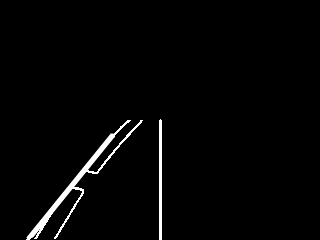
\includegraphics[width=0.7\textwidth]{03_Loesungskonzept/pictures/Fahrbahnlinien.png}
\caption{Eingetragene Fahrbahngrenze}
\label{fig:routeLimits}
\end{figure}
Um die Fahrtrichtung zu prüfen werden nun die ermittelten Fahrbahnlinien ausgewertet. Wenn beide Fahrbahnseiten erkannt werden, wird der Mittelwert aus beiden genutzt, ansonsten jeweils die vorhandene Seite. Die Auswertung erfolgt nach folgenden Schritten:
\begin{enumerate}
\item Verzerrungskorrektur rechnen: Da schräg auf die Fahrbahn geschaut wird, ist die Fahrbahn nicht parallel sondern entsprechend gegen die Bildrichtung zusammenlaufend. Dies wird für die Abstandsermittlung berücksichtigt. Der Neigungswinkel der Kamera ist so gewählt, dass die Korrektur mit folgender, einfacher Formel berechnet werden kann:
\[
D = \frac{y}{2} + 40 
\]
Wobei $D$ der Solldistanz und $y$ der höheren Bildzeile der Linie entspricht. Diese Formel ist nur gültig, da bei gerader Fahrbahn die Differenz zwischen oberer und unterer Distanz der Fahrbahnlinien exakt der Hälfte der Bildhöhe entspricht (Abbildung: \ref{fig:routeCorr}).
\item Abstand mit Sollwert vergleichen und die Differenz ermitteln.
\item Den Winkel der Korrektur berechnen. Die Kamera schaut 200mm vor die Mitte der Vorderachse, was 160 Bildpixel entspricht.
\item Der ermittelte Korrekturwinkel wird an den PD-Regler weitergegeben, die detaillierte Übersicht folgt später in diesem Abschnitt.
\end{enumerate}
\begin{figure}[H]%Position festigen
\centering
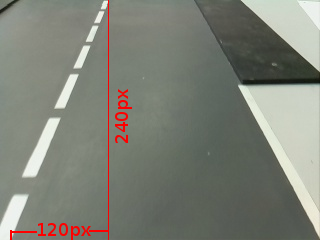
\includegraphics[width=0.7\textwidth]{03_Loesungskonzept/pictures/Verzerrung.png}
\caption{Verzerrung des Bildes}
\label{fig:routeCorr}
\end{figure}
Zugleich der Fahrbahnermittlung wird für jedes Bild die Steigung der Fahrbahnkanten überwacht. Unterschreiten diese die Mindestgrenze, wird eine Kurve erkannt und die Kamera auf einen Winkel von 20° bei Aussenkurven und 25° bei Innenkurven eingelenkt. Der Stellwert $s$ für den Servo kann unter Anwendung, dass 30° einer Stellwertdifferenz von 50 entspricht, wie folgt berechnet werden: 
\[
s = \frac{5}{3}\alpha_{cam}
\]
Entprechend wird die Solldistanz um den entsprechenden Pixelwert aus der Mitte versetzt um die veränderte Perspektive auszugleichen. Überschreitet die Steigung der Fahrbahnlinien die Obergrenze, wird die Kamera wieder auf die gerade Position zurückgeschwenkt. Der Korrekturwert $A$ lässt sich gemäss Schema in Abbildung \ref{fig:corrCam} mit folgender Formel approxximieren, die Abweichung vom Bogensegment zur Geraden ist vernachlässigbar klein:
\[
A \approx \frac{r\pi\alpha_{cam}}{180} \,, \text{ mit }r=160px = \frac{160\pi\alpha_{cam}}{180} = \frac{8}{9}\pi\alpha_{cam}
\]
\begin{figure}[H]%Position festigen
\centering
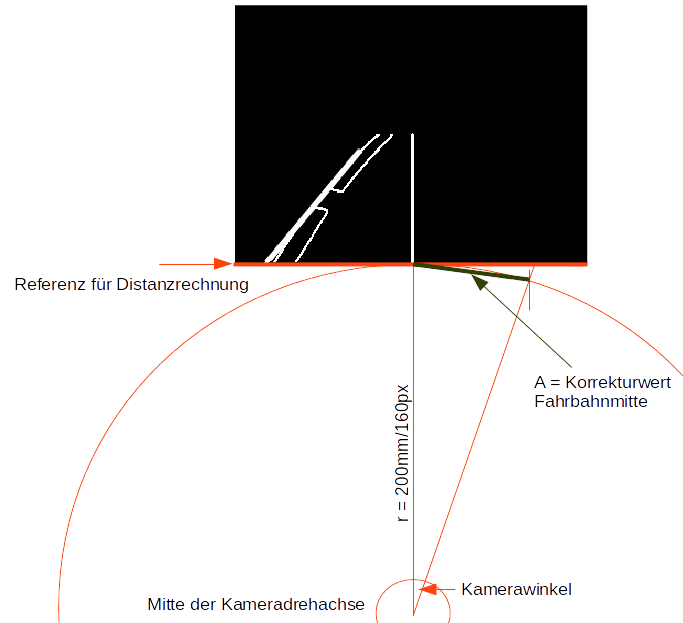
\includegraphics[width=0.7\textwidth]{03_Loesungskonzept/pictures/Kamerawinkelkorrektur.png}
\caption{Korrekturschema für den Kamerawinkel}
\label{fig:corrCam}
\end{figure}
Um zu Beginn ein Einlenken der Kamera zu verhindern wird diese Funktion erst nach einer gewissen Anzahl verarbeiteter Bilder aktiviert. Der Wert kann, wie auch die Unter- und Obergrenze der Steigung, in der Konfigurationsdatei festgelegt werden. 
Sobald die Fahrbahn erkannt ist, erhält der Controller den Auftrag zu fahren. Sollte die Fahrbahn verloren gehen, wird ein Counter aktiviert und eine in der Konfigurationsdatei einstellbare Anzahl Bilder in der letzten Richtung weitergefahren. Wird die Fahrbahn nicht wiedergefunden erhält der Controller die Information und stoppt das Programm.\\
Das Zielfeld und die Kreuzung werden anhand der Steigungen der Querlinien ermittelt. Wird eine Linie, mit entsprechender Länge identifiziert, erhält der Controller die entsprechende Information.
Die Parameter für die Regelung der Lenkung werden im Anschluss an die Winkelberechnung mit folgender Formel ermittelt:
\[
u(t) = K_p\left(T_v\frac{d}{dt}e(t) + e(t)\right)
\]
wobei $e(t)$ dem ermittelten Winkel entspricht. Im Anschluss wird der Stellwert $u(t)$ geprüft, ob er im zulässigen Bereich von $\pm 125$ entspricht. Über- oder unterschreitet $u(t)$ diese Grenze wird er entsprechend auf diese Limits korrigiert. Die Parameter $T_v$ (D-Anteil) und $K_{P}$ (P-Anteil) sind für die Feineinstellung justierbar und können in der Konfigurationsdatei festgelegt werden.
Die Erkennung der Kreuzungen und des Zielfeldes erfolgt parallel zur Fahrbahnerekennung und wird, da die Linien im Startbereich bewusst unbeachtet gelassen werden, gleichzeitig mit der Kurvenprüfung gestartet. Um eine Kreuzung zu akzeptieren werden folgende Filter verwendet:
\begin{itemize}
\item Es müssen sich mindestens vier Linien im Vektor befinden, die in der ersten Selektion die Steigung 0 aufweisen.
\item Ist die erste Bedingung erfüllt wird die Länge aller Linien berechnet. Ist diese grösser als 200 Pixel wird eine Querung registriert.
\item Werden fünf Querungen in Serie registriert wird eine Kreuzung gemeldet, und der Kruezungszaähler erhöht.
\end{itemize}
Im Anschluss wird eine Wartephase von 100 Bildern aktiviert. in dieser Zeit wird die Kreuzungserkennung ausgesetzt um die Ressourcen zu schonen. Im Zielbereich ist dann die Linie durchgezogen, das bedeutet die maximale Länge der Linien muss 300 Pixel betragen. Wird dieser Wert entsprechend dem Filter überschritten, wird das Ziel markiert und der Programmabschluss eingeleitet.\\[0.2cm]
\textbf{Vergleich Konzept und Umsetzung}\\[0.2cm]
Im Unterschied zum geplanten Konzept der Fahrbahnerkennung ist die Hough-Transformation für die Fahrbahnverankerung. Die Tests der ursprünglich geplanten Fahrbahnverankerung über ein Abtasten der Pixelwerte von innen nach aussen haben zu viele Störfaktoren aufgezeigt, wie kleine Risse in der Fahrbahn oder die Übergänge der Bauteile der Strecke. Deshalb ist an dieser Stelle eine Hough-Transformation implementiert. Diese Lösung hat sich als sehr robust erwiesen und die Filterung der Linien ermöglicht ein präzises aussortieren der Linien, die zu stark von der aktuellen Fahrtrichtung abweichen. Die ursprüngliche Befürchtung, die Hough-Transformation könnte zu viele Ressourcen beanspruchen, hat sich nach intensiven Tests als unbegründet herausgestellt. Die optimale Framerate von ca. 20 Bilder pro Sekunde kann eingehalten werden.\\
Weiter ist der Kantendetektionsalgorithmus leicht angepasst. Es wird neu über zwei Pixel hinweg geprüft und nicht nur über das unmittelbar benachbarte Pixel. Diese Änderung hat eine Erhöhung des Schwellwertes für den Gradienten ermöglicht was zu kleineren Bildstörungen durch Kratzer oder Spiegelungen führt.\\
Ein weitere Abweichung zum ursprünglichen Konzept ist die Regelung der Lenkung. Im Verlaufe der Tests ist der I-Antel des PID-Reglers auf 0 gesetzt worden und somit ein PD-Regler entstanden. Dies aufgrund der ausreichenden Trägheit des Lenkungssystems, was eine Dämpfung des Reglers unnötig werden lässt.\\[0.2cm]
\textbf{Bewertung}\\[0.2cm]
Die Fahrbahnerkennung hat sich als robust und Bildstörungsresistent erwiesen. Die Realisierung ist komplex, da diverse Parameter beachtet und eingestellt werden müssen um ein optimales Resultat zu erhalten. Die gewählte Kameraposition ermöglicht es, vorausschauend zu fahren, da ein grösserer Bereich vor dem Fahrzeug betrachtet wird. Zudem ist der Einsatz von weiteren Kameras nicht notwendig, da auch die Objekterkennung über die gleiche Bildquelle möglich ist.
\newpage
\underline{\textbf{Fahrbahnerkennung Unterstützung}}\\[0.2cm]
Unterstützend zur Kameraauswertung hat die Steuerung noch eine weitere Angabe zur Verfügung. Dies ist die gemessene Distanz des Fahrzeuges zum Gehsteig. Dies wird über den Flexsensor realisiert. Wie in der Dokumentation von Pren1 erläutert, ändert der Flexsensor seinen Widerstandswert je nachdem wie fest der Sensor gebogen ist. Der Widerstandswert wird über den Analog-Digitalwandler in dem Mikrocontroller eingelesen. Beim Einlesen dieses Wertes wurde festgestellt, dass dieser relativ grosses Rauschen enthält. Verursacht wurde dieses Rauschen hauptsächlich von der 5V Speisung. Diese enthält selbst gewisse Störungen, welche nachher den Messwert beeinflussen. Gelöst wurde dieses Problem indem zusätzlich zum Flexsensorwert auch ein Spannungswert relativ zur Speisung eingelesen wird. Aus diesen beiden Messwerte kann das differentielle Signal berechnet werden, aus dem die Störungen am 5V Netz weniger Einfluss haben. Mit dem bereinigtem Signal kann nun der ungefähre Abstand zum Gehsteig berechnet werden. Dies geschieht über eine lineare Funktion. Die Umrechnung vom Widerstandswert zum Abstand stimmt somit nicht sehr genau, sollte aber als Zusatzinformation so reichen.%Todo Führ Bild vom montiertem Flexsensor ein.
\\[0.2cm]
\textbf{Vergleich Konzept und Umsetzung}\\[0.2cm]
Das Konzept wurde für den Flexsensor nicht verändert. Dieser war immer als Hilfswert gedacht und dies wurde nun auch so implementiert. Angepasst wurde lediglich die Messmethode, welche nun differentiell geschieht.